\documentclass[tikz,border=4pt]{standalone}
\usepackage{amsmath,amssymb}
\usetikzlibrary{arrows.meta}
\definecolor{navy}{HTML}{17365D}
\definecolor{xaxis}{HTML}{B6252D}
\definecolor{yaxis}{HTML}{217A3C}
\definecolor{zaxis}{HTML}{215AAB}
% One continuous opaque gripper body, with no drawn internal edge lines.
% Fingers remain downward. A further positive yaw makes its open face look right.
% R_z(110 deg) is illustrative geometry, not an experimental angle.
\newcommand{\PoseGripper}{%
  \pgfmathsetmacro{\GripYaw}{110}
  \pgfmathsetmacro{\GripXX}{cos(\GripYaw)-0.55*sin(\GripYaw)}
  \pgfmathsetmacro{\GripXY}{-0.42*sin(\GripYaw)}
  \pgfmathsetmacro{\GripYX}{-sin(\GripYaw)-0.55*cos(\GripYaw)}
  \pgfmathsetmacro{\GripYY}{-0.42*cos(\GripYaw)}
  \begin{scope}[x={(\GripXX cm,\GripXY cm)},
    y={(\GripYX cm,\GripYY cm)},z={(0cm,1cm)}]
    % Visible side faces of the same extruded body; flat fills without strokes.
    \path[fill=black!42]
      (-0.23,-0.14,-0.38)--(-0.23,0.14,-0.38)
      --(-0.23,0.14,0.48)--(-0.23,-0.14,0.48)--cycle;
    \path[fill=black!42]
      (0.42,-0.14,-0.38)--(0.42,0.14,-0.38)
      --(0.42,0.14,0.90)--(0.42,-0.14,0.90)--cycle;
    \path[fill=black!12]
      (0.42,-0.14,0.90)--(0.42,0.14,0.90)
      --(0.16,0.14,0.90)--(0.16,-0.14,0.90)--cycle;
    \path[fill=black!42]
      (0.16,-0.14,0.90)--(0.16,0.14,0.90)
      --(0.16,0.14,1.13)--(0.16,-0.14,1.13)--cycle;
    \path[fill=black!12]
      (0.16,-0.14,1.13)--(0.16,0.14,1.13)
      --(-0.16,0.14,1.13)--(-0.16,-0.14,1.13)--cycle;
    \path[fill=black!12]
      (-0.16,-0.14,0.90)--(-0.16,0.14,0.90)
      --(-0.42,0.14,0.90)--(-0.42,-0.14,0.90)--cycle;
    % A single filled contour joins both fingers, palm and wrist.
    \path[fill=black!27]
      (-0.42,-0.14,-0.38)--(-0.23,-0.14,-0.38)
      --(-0.23,-0.14,0.48)--(0.23,-0.14,0.48)
      --(0.23,-0.14,-0.38)--(0.42,-0.14,-0.38)
      --(0.42,-0.14,0.90)--(0.16,-0.14,0.90)
      --(0.16,-0.14,1.13)--(-0.16,-0.14,1.13)
      --(-0.16,-0.14,0.90)--(-0.42,-0.14,0.90)--cycle;
  \end{scope}
}

\begin{document}
% Illustrative positive rotations around reference axes. Roll--pitch--yaw
% convention in notes: R = R_z(psi) R_y(theta) R_x(phi).
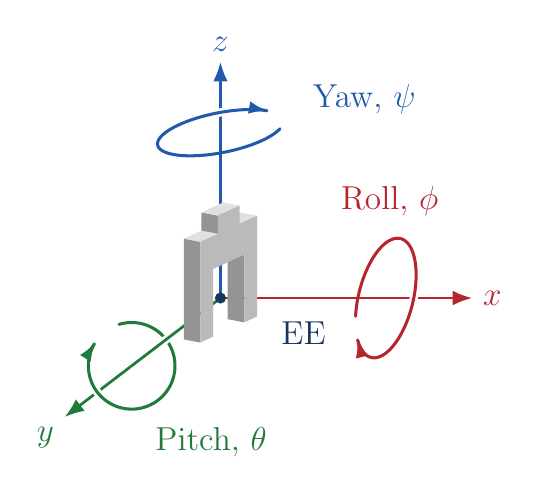
\begin{tikzpicture}[x={(1cm,0cm)},y={(-0.55cm,-0.42cm)},z={(0cm,1cm)},
 font=\large,axis/.style={-{Latex[length=2.5mm]},line width=1pt},
 % Rotation curls are sampled as fine polylines rather than smoothed plots, so
 % every arrow tip stays exactly tangent to the ring it closes. Ring radii are
 % kept well above the tip length so the heads follow the arcs.
 curl/.style={line width=1.1pt,line cap=round,line join=round,
   samples=140,variable=\t},
 curltip/.style={-{Latex[length=2.4mm,width=1.6mm]}},
 % White casing under whichever part of a ring passes in front of its own axis.
 casing/.style={white,line width=3pt,line cap=butt,line join=round,
   samples=140,variable=\t}]

% Right-hand rotations: x sends y toward z; y sends z toward x; z sends x
% toward y. Each ring is split where it crosses its own axis. The half on the
% far side is drawn before the axes and the near half after them over a white
% casing, so the axis passes through each ring instead of over it.
\draw[curl,zaxis,domain=350:500] plot ({0.7*cos(\t)},{0.7*sin(\t)},2.1);
\draw[curl,xaxis,domain=5:115] plot (2.1,{0.7*cos(\t)},{0.7*sin(\t)});

% Reference axes start at EE; the opaque gripper hides the portions behind it.
\draw[axis,xaxis] (0,0,0)--(3.2,0,0) node[right] {$x$};
\draw[axis,yaxis] (0,0,0)--(0,3.6,0) node[below left] {$y$};
\draw[axis,zaxis] (0,0,0)--(0,0,3) node[above] {$z$};

% The pitch ring lies in a plane of constant y, so its axis runs in front of the
% ring on the origin side and behind it on the far side.
\draw[casing,domain=343:663] plot ({0.55*sin(\t)},2.05,{0.55*cos(\t)});
\draw[curl,curltip,yaxis,domain=343:663]
 plot ({0.55*sin(\t)},2.05,{0.55*cos(\t)});
\draw[white,line width=3pt,line cap=butt] (0,1.15,0)--(0,2.07,0);
\draw[yaxis,line width=1pt,line cap=butt] (0,1.15,0)--(0,2.07,0);

\PoseGripper
\fill[navy] (0,0,0) circle (2.0pt);
\node[anchor=west,navy] at (0.65,0,-0.45) {EE};

\draw[casing,domain=498:650] plot ({0.7*cos(\t)},{0.7*sin(\t)},2.1);
\draw[curl,curltip,zaxis,domain=498:650]
 plot ({0.7*cos(\t)},{0.7*sin(\t)},2.1);
\draw[casing,domain=113:340] plot (2.1,{0.7*cos(\t)},{0.7*sin(\t)});
\draw[curl,curltip,xaxis,domain=113:340]
 plot (2.1,{0.7*cos(\t)},{0.7*sin(\t)});

% Labels sit clear of the rings and of the axis tips.
\node[xaxis,anchor=south] at (2.15,0,0.92) {Roll, $\phi$};
\node[yaxis,anchor=north west] at (-0.95,0,-1.52) {Pitch, $\theta$};
\node[zaxis,anchor=west] at (1.05,0,2.52) {Yaw, $\psi$};
\end{tikzpicture}
\end{document}
